\chapter{Discussion}

\section{Accuracy}

Our approach covered in this capstone report consists of two main parts: proposing a double-sided ArUco board as the calibration target and applying General Graph Optimisation (G2O) to enhance the accuracy of the calibration result.

In terms of the double-sided ArUco board, experiments have shown that this approach worked well in our project scope. All 16 cameras in our system could thoroughly detect the double-sided ArUco board in their field of view, and then our program framework could estimate the board's poses which are respected to each camera. Moreover, Open-CV library's solvePnP() function can calculate the transformation that minimises the re-projection errors and guarantees accuracy of the calibration results. To improve the calibration result with our approach, we suggest increasing the number of ArUco markers on both sides as well as their dimension; the more ArUco tags captured and detected by the camera, the higher the accuracy of the relative pose estimated.

On the other hand, the final extrinsic parameters are also calculated very accurately after finishing the pose graph optimisation process. The residual errors for total edges of the pose graph before optimising is 335.4759 millimetres, being significantly reduced to 16.90129 millimetres after optimising. Considering our pose graph has a total number of 1849 edges, the average residual error is just 0.009 millimetres per edge. This value can be regarded as an acceptable error. If possible, we recommend increasing the number of nodes in the pose graph by capturing more images, and it will help enhance the result of the optimisation process.

\begin{figure}[h]
\centering
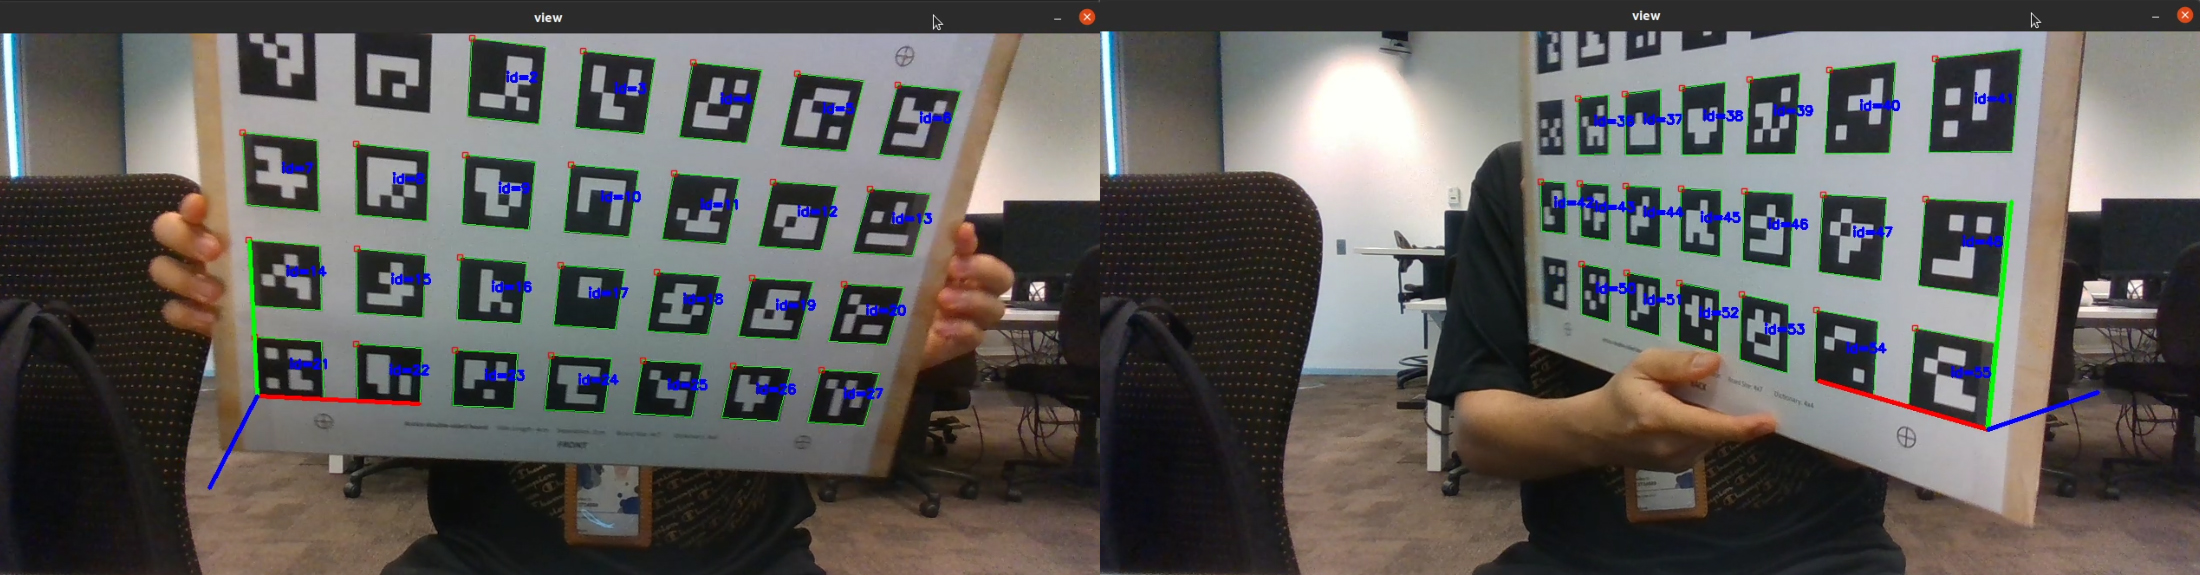
\includegraphics[width=1\textwidth]{Images/Board detection (both sides).jpg}
\caption{ArUco board estimation (both sides)}
\end{figure}

\begin{figure}[h]
\centering
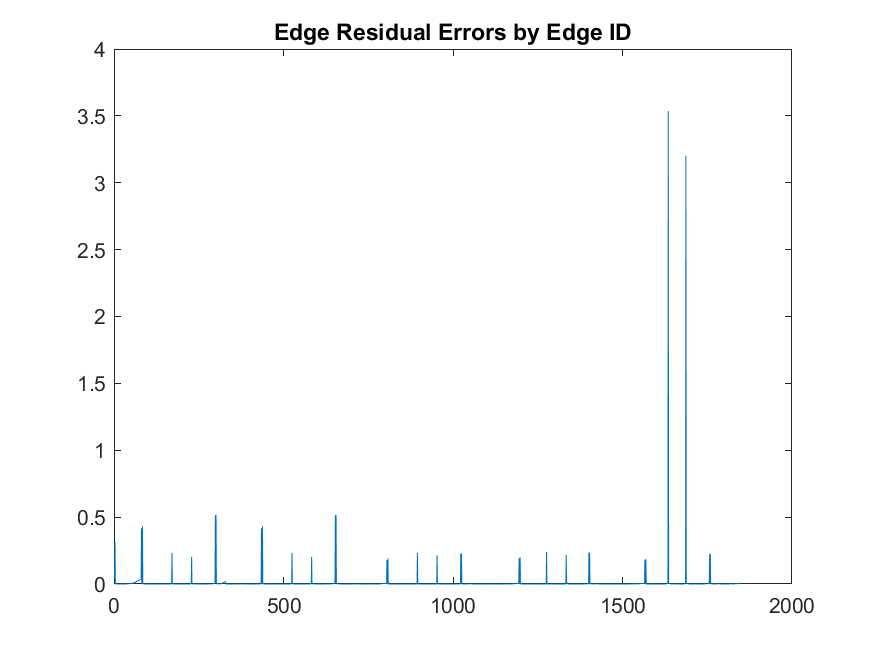
\includegraphics[width=1\textwidth]{Images/Edge Residual Errors by Edge ID.png}
\caption{Edge Residual Errors by Edge ID}
\end{figure}

% \clearpage
% \section{Uncertainties and difficulties}
% The first difficulty we faced during working on this project was the synchronisation of the multiple camera system. Each camera in the system will capture images independently with a frequency of about 30 Hz, which means the interval between each shot is about 33 ms. To apply the General Graph Optimisation, we have to ensure that at least two cameras have captured the ArUco board at the same timestamp. Therefore, we had to deal with the synchronisation of the multi-camera system.


\clearpage
\section{Further works}

We have only demonstrated the calibration of four cameras, but the entire system contains sixteen. Complete calibration of all cameras requires synchronisation of images with the reference camera, which needs to be tested. Furthermore, increasing the number of cameras may affect the convergence of the optimisation and final accuracy of the calibration results. Testing will need to be carried out to exclude board poses with fewer edges, i.e. fewer cameras see the board in that pose.

Currently, there is no way of getting ground truth poses between the cameras with the physical camera system. Therefore, we can not quantitatively test the accuracy of the estimated poses from our method. It may be possible to set up a simulator with multiple cameras, where the pose between the cameras is known, to test the calibration procedure. Noise can be added to images to replicate the functionality of physical cameras. Our calibration approach could also be tested with existing methods to compare results.

An important quantity that has not been considered is the uncertainty of our calibration parameters arising from the propagation of sensor noise. The calibration method relies on detecting fiducial markers in noisy images of the calibration board. The corners, in pixel coordinates, that are used in the optimisation will have some associated uncertainty. This uncertainty will be carried through the estimation of the board poses, and through the graph-based optimisation. Estimating the uncertainty can help us to understand the reliability of the final calibrated parameters, and potentially guide the collection of new images from cameras with high uncertainty. In completing this task, there is a possibility to publish the findings to a research conference.

Additionally, we would like to integrate the Pose Graph Optimisation into our program framework, so we will not need to save the relative pose between the ArUco board and each camera to CSV files, then run the MATLAB script for the optimisation. The General Graph Optimisation (G2O) algorithm will be coded in C++ and directly integrated into our framework, and then the optimisation process will be automatically run after finishing the board detection process for each camera. Besides, we would like to modify our program framework to be more modular to improve the processing speed and efficiency of the program. We will publish our framework in a public repository on GitHub and as an open-source ROS package for users.